% Part I — General Properties of Estimators
\section{General Properties of Estimators}

% \begin{frame}{Estimator Bias — definition, intuition, visual}
%   \textbf{Formal definition.}
%   For a parameter $\theta$ and estimator $\hat\theta$,
%   \[
%     \operatorname{Bias}_\theta(\hat\theta)\;=\;\mathbb{E}_\theta[\hat\theta] - \theta.
%   \]
%   In the vector case ($\theta\in\mathbb{R}^k$): $\operatorname{Bias}(\hat\theta)=\mathbb{E}[\hat\theta]-\theta$ (a $k$-vector).

%   \medskip
%   \textbf{Intuition (example).}
%   Bias is a \emph{systematic shift} from the truth.
%   Example: the ``MLE'' sample variance
%   $\widehat{\sigma}^2_{\,\text{MLE}}=\frac1n\sum_{i=1}^n (X_i-\bar X)^2$
%   is biased for $\sigma^2$; the unbiased version divides by $n-1$.

%   \medskip
%   \textbf{Visual (biased vs unbiased):}
%   \begin{center}
%   \begin{tikzpicture}[scale=0.9]
%     % axis
%     \draw[-{Stealth[length=3pt]}] (-3.5,0) -- (3.8,0) node[right] {$\theta$-axis};
%     % true theta
%     \draw[red, thick] (0,-0.02) -- (0,0.12) node[above, yshift=2pt] {$\theta$ (truth)};
%     % unbiased bell (centered)
%     \draw[blue, thick, opacity=0.9, domain=-3:3, samples=120]
%       plot (\x, {0.35*exp(-(\x)^2/1.2)});
%     \node[blue] at (1.9,0.35*exp(-(1.9)^2/1.2)) {\scriptsize unbiased};
%     % biased bell (shifted right)
%     \draw[orange, thick, opacity=0.9, domain=-3:3, samples=120, yshift=0cm]
%       plot (\x, {0.35*exp(-(\x-1)^2/1.2)});
%     \node[orange] at (2.5,0.35*exp(-((2.5-1)^2)/1.2)) {\scriptsize biased ($>0$)};
%     % mean markers
%     \draw[blue] (0,-0.02) -- (0,0.22);
%     \draw[orange] (1,-0.02) -- (1,0.22) node[above, yshift=2pt] {$\mathbb{E}[\hat\theta]$};
%   \end{tikzpicture}
%   \end{center}
% \end{frame}


% Slide 1 — Motivation
\begin{frame}{Why study estimator properties?}
  \begin{itemize}
  \item Not all estimators are equal \(\to\) need tools to choose the "best" one
    \item Helps decide between MLE, MoM, or others in practice
    \item Key question: \textbf{Which estimator should we trust?}
  \end{itemize}

  \vspace{1em}
  % Visual moved to a dedicated frame to avoid overflow
\end{frame}

% Visual frame — Why study estimator properties?
\begin{frame}{Why study estimator properties? -- Visual}
  \begin{center}
    \begin{adjustbox}{max height=0.40\textheight}
    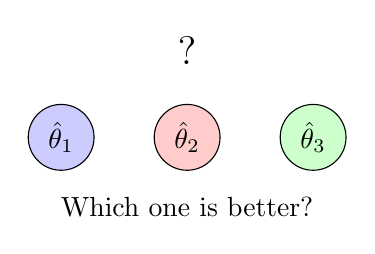
\begin{tikzpicture}[scale=0.8]
      % Multiple estimators competing
      \node[draw, circle, fill=blue!20] at (0,0) {$\hat{\theta}_1$};
      \node[draw, circle, fill=red!20] at (2,0) {$\hat{\theta}_2$};
      \node[draw, circle, fill=green!20] at (4,0) {$\hat{\theta}_3$};
      \node[above, font=\Large] at (2,1) {?};
      \node[below] at (2,-0.8) {Which one is better?};
    \end{tikzpicture}
    \end{adjustbox}
  \end{center}
\end{frame}

% Slide 2 — Bias
\begin{frame}{Bias}
  \begin{block}{Definition}
    The bias of an estimator is
    \[\Bias(\hat{\theta}) = \E[\hat{\theta}] - \theta.\]
  \end{block}

  \begin{block}{Intuition}
    Bias measures systematic error: if non-zero the estimator is centered away
    from the true parameter even as we average over repeated samples. In practice
    bias affects accuracy and may require correction or a bias--variance tradeoff.
  \end{block}

  \vspace{1em}
  % Visual moved to its own slide
\end{frame}

% Visual frame — Bias (visual)
\begin{frame}{Bias -- Visual}
  \begin{center}
    \begin{adjustbox}{max height=0.40\textheight}
    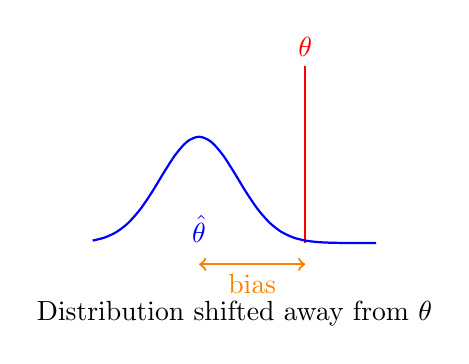
\begin{tikzpicture}[scale=0.9]
      % True parameter
      \draw[thick, red] (3, 0) -- (3, 2.5);
      \node[red, above] at (3, 2.5) {$\theta$};

      % Biased estimator distribution
      \draw[blue, thick, domain=0:4, smooth] plot (\x, {1.5*exp(-0.5*(\x-1.5)^2/0.3)});
      \node[blue] at (1.5, 0.2) {$\hat{\theta}$};

      % Arrow showing bias
      \draw[<->, thick, orange] (1.5, -0.3) -- (3, -0.3);
      \node[orange, below] at (2.25, -0.3) {bias};

      \node at (2, -1) {Distribution shifted away from $\theta$};
    \end{tikzpicture}
    \end{adjustbox}
  \end{center}
\end{frame}

% Slide 3 — Variance
\begin{frame}{Variance}
  \begin{block}{Definition}
    The variance of an estimator is
    \[\Var(\hat{\theta}) = \E\big[(\hat{\theta} - \E[\hat{\theta}])^2\big].\]
  \end{block}

  \begin{block}{Intuition}
    Variance measures randomness in the estimator across different samples.
    Low variance means repeated experiments produce similar estimates; high
    variance implies lack of precision. For practitioners, variance controls
    confidence interval width and sample size planning.
  \end{block}

  \vspace{1em}
  % Visual only; split to avoid overflow
\end{frame}

% Visual frame — Variance (visual)
\begin{frame}{Variance -- Visual}
  \begin{center}
    \begin{adjustbox}{max height=0.40\textheight}
    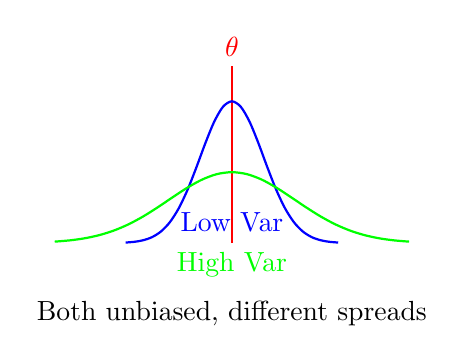
\begin{tikzpicture}[scale=0.9]
      % True parameter
      \draw[thick, red] (3, 0) -- (3, 2.5);
      \node[red, above] at (3, 2.5) {$\theta$};

      % Low variance estimator
      \draw[blue, thick, domain=1.5:4.5, smooth] plot (\x, {2*exp(-0.5*(\x-3)^2/0.2)});
      \node[blue] at (3, 0.3) {Low Var};

      % High variance estimator
      \draw[green, thick, domain=0.5:5.5, smooth] plot (\x, {1*exp(-0.5*(\x-3)^2/0.8)});
      \node[green] at (3, -0.3) {High Var};

      \node at (3, -1) {Both unbiased, different spreads};
    \end{tikzpicture}
    \end{adjustbox}
  \end{center}
\end{frame}

% Slide 4 — MSE & Bias-Variance Tradeoff
\begin{frame}{MSE and Bias--Variance Tradeoff}
  \begin{block}{Definition}
    The mean squared error of an estimator is
    \[\MSE(\hat{\theta}) = \E\big[(\hat{\theta} - \theta)^2\big].\]
    It decomposes as
    \[\MSE(\hat{\theta}) = \Bias(\hat{\theta})^2 + \Var(\hat{\theta}).\]
  \end{block}

  \begin{block}{Intuition}
    MSE trades off accuracy (bias) against precision (variance). In applied work
    a small bias can be acceptable if it substantially reduces variance and
    thereby improves prediction or interval width.
  \end{block}

      \vspace{1em}
          % Visual moved to separate frame below to avoid overflow
      \end{frame}

      % Visual frame — MSE and Tradeoff (visual)
      \begin{frame}{MSE and Bias--Variance Tradeoff -- Visual}
        \begin{center}
          \begin{adjustbox}{max height=0.40\textheight}
          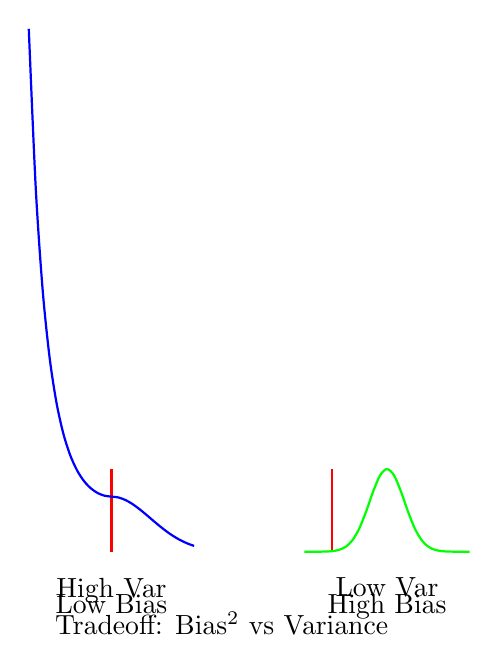
\begin{tikzpicture}[scale=0.7]
            % High variance, low bias
            \begin{scope}[xshift=-2cm]
              \draw[thick, red] (0, 0) -- (0, 1.5);
              \draw[blue, thick, domain=-1.5:1.5, smooth] plot (\x, {exp(-0.5*\x^2/0.5)});
              \node[below] at (0, -0.3) {High Var};
              \node[below] at (0, -0.6) {Low Bias};
            \end{scope}

            % Low variance, high bias
            \begin{scope}[xshift=2cm]
              \draw[thick, red] (0, 0) -- (0, 1.5);
              \draw[green, thick, domain=-0.5:2.5, smooth] plot (\x, {1.5*exp(-0.5*(\x-1)^2/0.1)});
              \node[below] at (1, -0.3) {Low Var};
              \node[below] at (1, -0.6) {High Bias};
            \end{scope}

            \node at (0, -1.3) {Tradeoff: Bias$^2$ vs Variance};
          \end{tikzpicture}
          \end{adjustbox}
        \end{center}
      \end{frame}

% Slide 5 — Consistency
\begin{frame}{Consistency}
  \begin{block}{Definition}
    An estimator $\hat{\theta}_n$ is consistent for $\theta$ if
    \[\hat{\theta}_n \xrightarrow{\;\mathsf{P}\;} \theta \qquad (n \to \infty).
    \]
  \end{block}

  \begin{block}{Intuition}
    With increasing sample size the estimator concentrates around the true
    value. Consistency is a minimal long-run requirement: without it an
    estimator may never learn the truth no matter how much data you collect.
  \end{block}

  \vspace{1em}
  \begin{center}
    % Visual moved to its own frame below
  \end{center}
\end{frame}

% Visual frame — Consistency (visual)
\begin{frame}{Consistency -- Visual}
  \begin{center}
    \begin{adjustbox}{max height=0.40\textheight}
    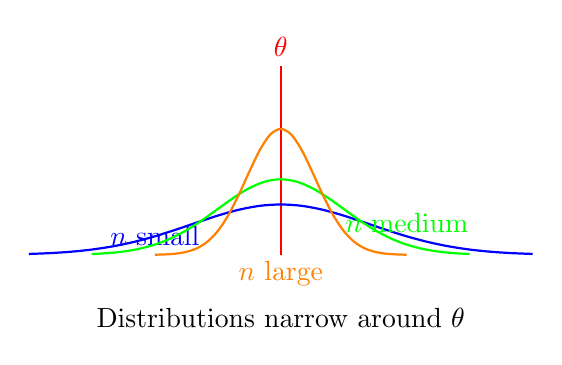
\begin{tikzpicture}[scale=0.8]
      % True parameter
      \draw[thick, red] (4, 0) -- (4, 3);
      \node[red, above] at (4, 3) {$\theta$};

      % Sequence of distributions narrowing
      \draw[blue, thick, domain=0:8, smooth] plot (\x, {0.8*exp(-0.5*(\x-4)^2/2)});
      \node[blue] at (2, 0.3) {$n$ small};

      \draw[green, thick, domain=1:7, smooth] plot (\x, {1.2*exp(-0.5*(\x-4)^2/1)});
      \node[green] at (6, 0.5) {$n$ medium};

      \draw[orange, thick, domain=2:6, smooth] plot (\x, {2*exp(-0.5*(\x-4)^2/0.3)});
      \node[orange] at (4, -0.3) {$n$ large};

      \node at (4, -1) {Distributions narrow around $\theta$};
    \end{tikzpicture}
    \end{adjustbox}
  \end{center}
\end{frame}

% Slide 6 — Asymptotic Normality
\begin{frame}{Asymptotic Normality}
  \begin{block}{Definition}
    An estimator satisfies asymptotic normality when
    \[\sqrt{n}(\hat{\theta} - \theta) \xrightarrow{\;\mathcal{D}\;} N(0,\sigma^2),\]
    i.e. the rescaled error converges in distribution to a Gaussian.
  \end{block}

  \begin{block}{Intuition}
    For large samples the estimator's sampling distribution becomes approximately
    normal. This justifies using Wald-style confidence intervals and tests in
    applied work even when the exact small-sample distribution is unknown.
  \end{block}

  \vspace{1em}
  \begin{center}
    % Visual moved below
  \end{center}
\end{frame}

% Visual frame — Asymptotic Normality (visual)
\begin{frame}{Asymptotic Normality -- Visual}
  \begin{center}
    \begin{adjustbox}{max height=0.40\textheight}
    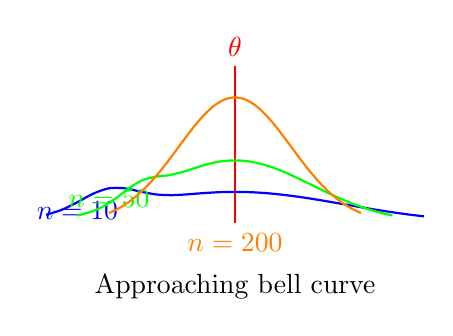
\begin{tikzpicture}[scale=0.8]
      % True parameter
      \draw[thick, red] (4, 0) -- (4, 2.5);
      \node[red, above] at (4, 2.5) {$\theta$};

      % Evolution to normal distribution
      \draw[blue, thick, domain=1:7, smooth] plot (\x, {0.5*exp(-0.5*(\x-4)^2/3) + 0.3*exp(-0.5*(\x-2)^2/0.2)});
      \node[blue] at (1.5, 0.2) {$n=10$};

      \draw[green, thick, domain=1.5:6.5, smooth] plot (\x, {exp(-0.5*(\x-4)^2/1.5) + 0.2*exp(-0.5*(\x-2.5)^2/0.1)});
      \node[green] at (2, 0.4) {$n=50$};

      \draw[orange, thick, domain=2:6, smooth] plot (\x, {2*exp(-0.5*(\x-4)^2/0.8)});
      \node[orange] at (4, -0.3) {$n=200$};

      \node at (4, -1) {Approaching bell curve};
    \end{tikzpicture}
    \end{adjustbox}
  \end{center}
\end{frame}

% Slide 7 — Efficiency and Cramér--Rao Bound
\begin{frame}{Efficiency and Cramér--Rao Bound}
  \begin{block}{Definition}
    The Cramér--Rao lower bound (CRLB) states that for an unbiased estimator
    \[\Var(\hat{\theta}) \geq \frac{1}{I(\theta)},\]
    where $I(\theta)$ is the Fisher information.
  \end{block}

  \begin{block}{Intuition}
    Fisher information measures the amount of data-driven "sharpness" in the
    likelihood: more information implies a tighter lower bound on variance.
    Efficient estimators asymptotically attain this bound; in applied work the
    CRLB helps set expectations about the best possible precision.
  \end{block}

  \vspace{1em}
  \begin{center}
    % Visual below
  \end{center}
\end{frame}

% Visual frame — Efficiency and Cram\'er--Rao Bound (visual)
\begin{frame}{Efficiency and Cram\'er--Rao Bound -- Visual}
  \begin{center}
    \begin{adjustbox}{max height=0.40\textheight}
    \begin{tikzpicture}[scale=0.8]
      % Flat likelihood (low info)
      \begin{scope}[xshift=-2cm]
        \draw[blue, thick, domain=-1.5:1.5, smooth] plot (\x, {0.8 - 0.1*\x^2});
        \node[below] at (0, -0.3) {Flat likelihood};
        \node[below] at (0, -0.6) {Low info, high var};
      \end{scope}

      % Sharp likelihood (high info)
      \begin{scope}[xshift=2cm]
        \draw[red, thick, domain=-1.5:1.5, smooth] plot (\x, {1.5*exp(-0.5*\x^2/0.2)});
        \node[below] at (0, -0.3) {Sharp likelihood};
        \node[below] at (0, -0.6) {High info, low var};
      \end{scope}

      \node at (0, -1.3) {Fisher Information vs Variance};
    \end{tikzpicture}
    \end{adjustbox}
  \end{center}
\end{frame}